\documentclass{article}

\usepackage{amsmath}  %% mathematics
\usepackage{graphicx}  %% graphics
\usepackage{caption,booktabs,threeparttable}  %% table with footnotes (see Table 2)
\usepackage{url}  %% Need for web address -- eg. in the bibliography for website cited

%%%%%%%%%%%%%%%%%%%%%%%%%%%%%%%%%%%%%%%%%%%%%%%%%%%%%%%%%%%
\title{Examples of Latex Code}
\author{Karl N. Kirschner}
\date{\today}

%%%%%%%%%%%%%%%%%%%%%%%%%%%%%%%%%%%%%%%%%%%%%%%%%%%%%%%%%%%
\begin{document}
\maketitle

%%%%%%%%%%%%%%%%%%%%%%%%%%%%%%%%%%%%%%%%%%%%%%%%%%%%%%%%%%%
\section{Indents, new lines and notes within document}
%% Comments within the text that is not compiled

%% Force a carriage return (also done with a blank line inbetween):
Hello world! \\
Hello moon!

%% Notice the indentation that results here:
Hello mars!

%% Force no indentation:
\noindent
Hello venus!

%% Notice that a carriage return is not inforced here:
Hello Jupiter,
hello Saturn!

%% A way to enforce skipped lines
~\\
~\\

%% Once can even insert personal notes to the middle of a paragraph
Lorem ipsum dolor sit amet, consectetur adipiscing elit, sed do eiusmod tempor incididunt ut labore et dolore magna aliqua. Ut enim ad minim veniam, quis nostrud exercitation ullamco laboris nisi ut aliquip ex ea commodo consequat. Duis aute irure dolor in reprehenderit in voluptate velit esse cillum dolore eu fugiat nulla pariatur.
%% The above was done using the x methodology.
Excepteur sint occaecat cupidatat non proident, sunt in culpa qui officia deserunt mollit anim id est laborum.

%%%%%%%%%%%%%%%%%%%%%%%%%%%%%%%%%%%%%%%%%%%%%%%%%%%%%%%%%%%
\section{Math}

\begin{equation}
  1 + 2 = 3
\end{equation}

%% No numbering of equation
\begin{equation*}
  4 + 2 = 6
\end{equation*}

%% Alignment using & and complex math
\begin{align}
  f(x) &= x^2\\
  g(x) &= \frac{1}{x}\\
  F(x) &= \int^a_b \frac{1}{3}x^3
\end{align}

%% Matrix notation
\begin{equation}
  M=
  \begin{bmatrix}
    1 & 2 & 3 & 4 & 5 \\
    3 & 4 & 5 & 6 & 7
  \end{bmatrix}
\end{equation}

%%%%%%%%%%%%%%%%%%%%%%%%%%%%%%%%%%%%%%%%%%%%%%%%%%%%%%%%%%%
\section{Verbatim}

\begin{verbatim}
Lorem ipsum dolor sit amet, consectetur adipiscing elit,
sed do eiusmod tempor incididunt ut labore et dolore magna
aliqua. Ut enim ad minim veniam, quis nostrud exercitation
ullamco laboris nisi ut aliquip ex ea commodo consequat.
Duis aute irure dolor in reprehenderit in voluptate velit
esse cillum dolore eu               fugiat nulla pariatur.
Excepteur sint occaecat cupidatat non proident,
sunt in culpa qui officia deserunt mollit anim id est

laborum
\end{verbatim}

%%%%%%%%%%%%%%%%%%%%%%%%%%%%%%%%%%%%%%%%%%%%%%%%%%%%%%%%%%%
\section{Figures and referencing labels.}

In Figure \ref{fig:example1} one can see an example for a single figure. In Figure \ref{fig:example2} we see a side-by-side figure. If one wants subcaptions then take a look at the ``subcaption'' package for Latex.

\begin{figure*}[h!]
  \centering
  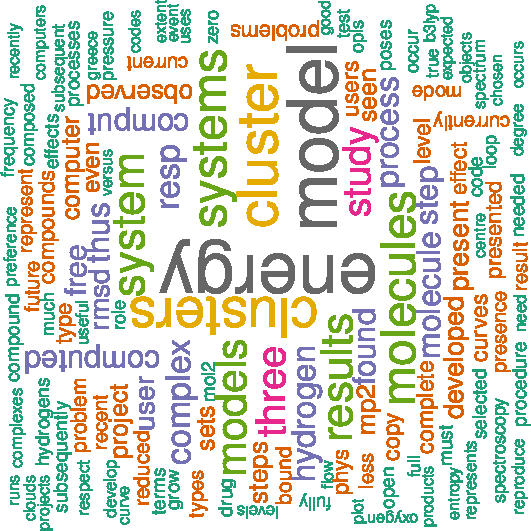
\includegraphics[width=4cm]{papers_2010_2015}
  \caption{Example figure number 1.}
  \label{fig:example1}
\end{figure*}

\begin{figure*}[h!]
  \centering
  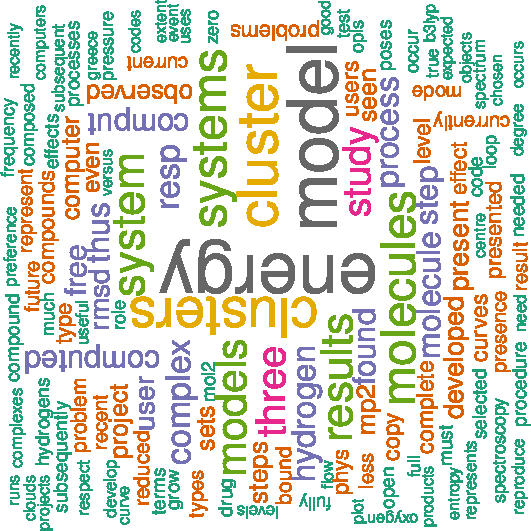
\includegraphics[width=0.30\linewidth]{papers_2010_2015}
  \hspace{1cm} %% horizontal space
  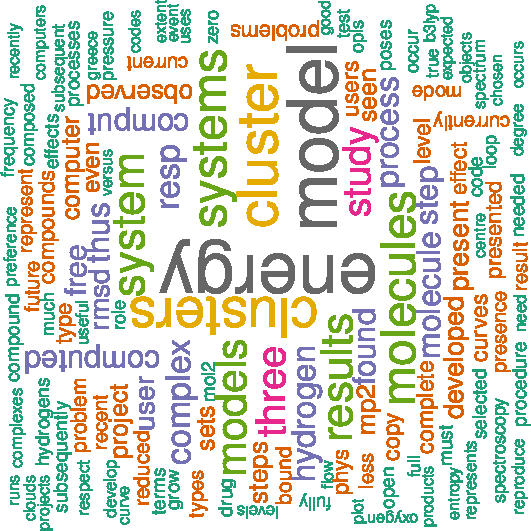
\includegraphics[width=0.30\linewidth]{papers_2010_2015}
  \caption{Example of a side-by-side figure number 2.}
  \label{fig:example2}
\end{figure*}

%%%%%%%%%%%%%%%%%%%%%%%%%%%%%%%%%%%%%%%%%%%%%%%%%%%%%%%%%%%
\section{Tables, bold face text and Greek letters}

Table \ref{tab:example1} shows a simple table, which does not require any special packages. If you want to add footnotes to your table, take a look at the Latex ``threeparttable'' package -- see Table \ref{tab:example2}.

\begin{table}[h!]
  \centering
  \caption{Example of a simple table.}
  \label{tab:example1}
  \normalsize  %% fontsize for table
  \begin{tabular}{l|cr}
      \hline \hline
      \multicolumn{3}{c}{\textbf{Some Bigger Header Goes Here}} \\
      \textbf{Some Items} & \textbf{Value of Item} & \textbf{Notation} \\
      \hline
      Item 1 & 1.001 & $\alpha$ \\
      Item 2 & 2.002 & $\beta$ \\
      Item 3 & 3.003 & $\gamma$ \\
      \hline \hline
  \end{tabular}
\end{table}

\begin{table}[!ht]
    \centering
    \begin{threeparttable}
	\captionsetup{font=Large,labelfont=bf,labelsep=period}
	\caption{Example of a simple table.}
	\label{tab:example2}
	\Large
	\begin{tabular}{l|cc}
	    \hline \hline
	    \multicolumn{3}{c}{\textbf{Some Bigger Header Goes Here}} \\
	    \textbf{Some Items} & \textbf{Value of Item} & \textbf{Notation} \\
	    \hline
	    Item 1 & 1.001 & $\alpha$ \\
	    Item 2 & 2.002 & $\beta$ \\
	    Item 3 & 3.003\tnote{a} & $\gamma$ \\
	    \hline \hline
	\end{tabular}
	\begin{tablenotes}
	    %\footnotesize
	    \item[a] Footnote
	\end{tablenotes}
    \end{threeparttable}
\end{table}

%%%%%%%%%%%%%%%%%%%%%%%%%%%%%%%%%%%%%%%%%%%%%%%%%%%%%%%%%%%
\newpage
\section{Citations}

Lorem ipsum dolor sit amet, consectetur adipiscing elit \cite{Baranac-StojanovicAS2015}, sed do eiusmod tempor incididunt ut labore \cite{AMBER16} et dolore magna aliqua. Ut enim ad minim veniam \cite{MartinP2001}, quis nostrud exercitation ullamco laboris nisi ut aliquip ex ea commodo consequat \cite{McQuarrie1976}. Duis aute irure dolor in reprehenderit in voluptate velit esse cillum dolore eu fugiat nulla pariatur \cite{PriemTGN2010}. Excepteur sint occaecat cupidatat non proident, sunt in culpa qui officia deserunt mollit anim id est laborum \cite{R}.

\bibliographystyle{abbrv}
\bibliography{bibtex_examples}
%%%%%%%%%%%%%%%%%%%%%%%%%%%%%%%%%%%%%%%%%%%%%%%%%%%%%%%%%%%
\end{document}
